% 1.6.2: tabel over mean+var over 10 runs + 
%        graf dpi vs success for filtre (10 run)

\subsection{Preprocessed Image - Single Person Tests}

\begin{table}[h]
\centering
    \begin{subtable}[b]{0.56\textwidth}
    \centering
        \begin{tabular}{lcccccc}
            &Raw	& Avg	& G 0.5	& G 1	& G 2 \\
\hline
100	& 0.8297	& 0.860	& 0.8297	& 0.8545	& 0.7750 \\
200	& 0.8635	& 0.895	& 0.8635	& 0.8998	& 0.8602 \\
300	& 0.8925	& 0.920	& 0.8925	& 0.9190	& 0.8842 \\

        \end{tabular}
        \caption{Mean success rate}
    \end{subtable}
    \begin{subtable}[b]{0.42\textwidth}
    \centering
        \begin{tabular}{lcccccc}
            &Raw	& Avg	& G 1	& G 2	& G 3 \\
\hline
100	& NA	& NA	& NA	& NA	& NA \\
200	& NA	& NA	& NA	& NA	& NA \\
300	& NA	& NA	& NA	& NA	& NA \\

        \end{tabular}
        \caption{Variance in success rate}
    \end{subtable}
    \caption[Success of smoothing functions]{Success mean and variance of different smoothing functions.}
    \label{tb:smooth}
\end{table}

\begin{figure}[h]
\centering
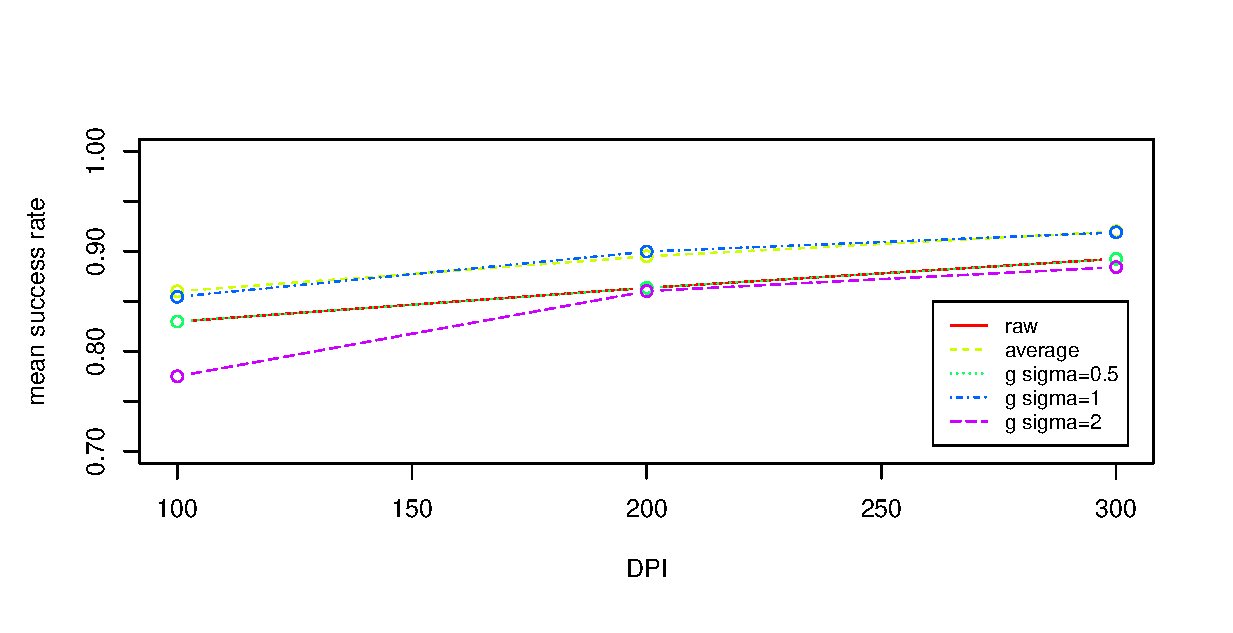
\includegraphics[width=1\textwidth]{graphics/smoothing}
\caption{Success of smoothing functions}
\label{fig:smooth}
\end{figure}

Applying a smoothing function can give the image an advantage when using the nearest neighbour analysis.
By taking an average of the neighbouring pixels the lines in the digit should be wider and the digits should have a better chance of overlapping.
The danger is that too much smoothing could make the whole image one colour and would completely destroy any chance of analysis.
A Gaussian distribution (also referred to as a normal distribution) a naturally occurring distribution that happens when a random result occurs around a mean. 
The $\sigma$ signifies the deviation. 
The 2d equation of a Gaussian distribution is shown in equation \ref{eq:gauss}. 
Using this to smooth an image will weigh the distance to the pixel.
A small $\sigma$ will make a small deviation and thus heavily weigh the center pixel.
To compare with no filter we have measured a raw image with 100, 200 and 300 DPI.
These results are compared with an averaging filter (avg) which takes the average of 4 neighbouring pixels and a Gaussian filter (G) with different sigma.
These tests were done 10 times and the mean of each success is plotted in figure \ref{fig:smooth}. 
Since the variance is too small to be seen in the graph the mean and variance is shown in table \ref{tb:smooth}.
The averaging filter does not give a measurable different result from not using a filter.
The Gaussian filter improves the success rate but a large $\sigma$ makes it worse.
\begin{equation}
G(x,y) = \frac{1}{2\pi \sigma^2} e^{- \frac{x^2+y^2}{2\sigma^2}} \label{eq:gauss}
\end{equation}